%% bare_jrnl.tex
%% V1.4b
%% 2015/08/26
%% by Michael Shell
%% see http://www.michaelshell.org/
%% for current contact information.
%%
%% This is a skeleton file demonstrating the use of IEEEtran.cls
%% (requires IEEEtran.cls version 1.8b or later) with an IEEE
%% journal paper.
%%
%% Support sites:
%% http://www.michaelshell.org/tex/ieeetran/
%% http://www.ctan.org/pkg/ieeetran
%% and
%% http://www.ieee.org/

%%*************************************************************************
%% Legal Notice:
%% This code is offered as-is without any warranty either expressed or
%% implied; without even the implied warranty of MERCHANTABILITY or
%% FITNESS FOR A PARTICULAR PURPOSE! 
%% User assumes all risk.
%% In no event shall the IEEE or any contributor to this code be liable for
%% any damages or losses, including, but not limited to, incidental,
%% consequential, or any other damages, resulting from the use or misuse
%% of any information contained here.
%%
%% All comments are the opinions of their respective authors and are not
%% necessarily endorsed by the IEEE.
%%
%% This work is distributed under the LaTeX Project Public License (LPPL)
%% ( http://www.latex-project.org/ ) version 1.3, and may be freely used,
%% distributed and modified. A copy of the LPPL, version 1.3, is included
%% in the base LaTeX documentation of all distributions of LaTeX released
%% 2003/12/01 or later.
%% Retain all contribution notices and credits.
%% ** Modified files should be clearly indicated as such, including  **
%% ** renaming them and changing author support contact information. **
%%*************************************************************************


% *** Authors should verify (and, if needed, correct) their LaTeX system  ***
% *** with the testflow diagnostic prior to trusting their LaTeX platform ***
% *** with production work. The IEEE's font choices and paper sizes can   ***
% *** trigger bugs that do not appear when using other class files.       ***                          ***
% The testflow support page is at:
% http://www.michaelshell.org/tex/testflow/



\documentclass[journal]{IEEEtran}
%
% If IEEEtran.cls has not been installed into the LaTeX system files,
% manually specify the path to it like:
% \documentclass[journal]{../sty/IEEEtran}





% Some very useful LaTeX packages include:
% (uncomment the ones you want to load)


% *** MISC UTILITY PACKAGES ***
%
%\usepackage{ifpdf}
% Heiko Oberdiek's ifpdf.sty is very useful if you need conditional
% compilation based on whether the output is pdf or dvi.
% usage:
% \ifpdf
%   % pdf code
% \else
%   % dvi code
% \fi
% The latest version of ifpdf.sty can be obtained from:
% http://www.ctan.org/pkg/ifpdf
% Also, note that IEEEtran.cls V1.7 and later provides a builtin
% \ifCLASSINFOpdf conditional that works the same way.
% When switching from latex to pdflatex and vice-versa, the compiler may
% have to be run twice to clear warning/error messages.






% *** CITATION PACKAGES ***
%
\usepackage{cite}
\usepackage{hyperref}
\usepackage{array}
% cite.sty was written by Donald Arseneau
% V1.6 and later of IEEEtran pre-defines the format of the cite.sty package
% \cite{} output to follow that of the IEEE. Loading the cite package will
% result in citation numbers being automatically sorted and properly
% "compressed/ranged". e.g., [1], [9], [2], [7], [5], [6] without using
% cite.sty will become [1], [2], [5]--[7], [9] using cite.sty. cite.sty's
% \cite will automatically add leading space, if needed. Use cite.sty's
% noadjust option (cite.sty V3.8 and later) if you want to turn this off
% such as if a citation ever needs to be enclosed in parenthesis.
% cite.sty is already installed on most LaTeX systems. Be sure and use
% version 5.0 (2009-03-20) and later if using hyperref.sty.
% The latest version can be obtained at:
% http://www.ctan.org/pkg/cite
% The documentation is contained in the cite.sty file itself.






% *** GRAPHICS RELATED PACKAGES ***
%
\ifCLASSINFOpdf{}
  \usepackage[pdftex]{graphicx}
  % declare the path(s) where your graphic files are
  % \graphicspath{{../pdf/}{../jpeg/}}
  % and their extensions so you won't have to specify these with
  % every instance of \includegraphics
  % \DeclareGraphicsExtensions{.pdf,.jpeg,.png}
\else
  % or other class option (dvipsone, dvipdf, if not using dvips). graphicx
  % will default to the driver specified in the system graphics.cfg if no
  % driver is specified.
  % \usepackage[dvips]{graphicx}
  % declare the path(s) where your graphic files are
  % \graphicspath{{../eps/}}
  % and their extensions so you won't have to specify these with
  % every instance of \includegraphics
  % \DeclareGraphicsExtensions{.eps}
\fi
% graphicx was written by David Carlisle and Sebastian Rahtz. It is
% required if you want graphics, photos, etc. graphicx.sty is already
% installed on most LaTeX systems. The latest version and documentation
% can be obtained at: 
% http://www.ctan.org/pkg/graphicx
% Another good source of documentation is "Using Imported Graphics in
% LaTeX2e" by Keith Reckdahl which can be found at:
% http://www.ctan.org/pkg/epslatex
%
% latex, and pdflatex in dvi mode, support graphics in encapsulated
% postscript (.eps) format. pdflatex in pdf mode supports graphics
% in .pdf, .jpeg, .png and .mps (metapost) formats. Users should ensure
% that all non-photo figures use a vector format (.eps, .pdf, .mps) and
% not a bitmapped formats (.jpeg, .png). The IEEE frowns on bitmapped formats
% which can result in "jaggedy"/blurry rendering of lines and letters as
% well as large increases in file sizes.
%
% You can find documentation about the pdfTeX application at:
% http://www.tug.org/applications/pdftex





% *** MATH PACKAGES ***
%
%\usepackage{amsmath}
% A popular package from the American Mathematical Society that provides
% many useful and powerful commands for dealing with mathematics.
%
% Note that the amsmath package sets \interdisplaylinepenalty to 10000
% thus preventing page breaks from occurring within multiline equations. Use:
%\interdisplaylinepenalty=2500
% after loading amsmath to restore such page breaks as IEEEtran.cls normally
% does. amsmath.sty is already installed on most LaTeX systems. The latest
% version and documentation can be obtained at:
% http://www.ctan.org/pkg/amsmath





% *** SPECIALIZED LIST PACKAGES ***
%
%\usepackage{algorithmic}
% algorithmic.sty was written by Peter Williams and Rogerio Brito.
% This package provides an algorithmic environment fo describing algorithms.
% You can use the algorithmic environment in-text or within a figure
% environment to provide for a floating algorithm. Do NOT use the algorithm
% floating environment provided by algorithm.sty (by the same authors) or
% algorithm2e.sty (by Christophe Fiorio) as the IEEE does not use dedicated
% algorithm float types and packages that provide these will not provide
% correct IEEE style captions. The latest version and documentation of
% algorithmic.sty can be obtained at:
% http://www.ctan.org/pkg/algorithms
% Also of interest may be the (relatively newer and more customizable)
% algorithmicx.sty package by Szasz Janos:
% http://www.ctan.org/pkg/algorithmicx




% *** ALIGNMENT PACKAGES ***
%
%\usepackage{array}
% Frank Mittelbach's and David Carlisle's array.sty patches and improves
% the standard LaTeX2e array and tabular environments to provide better
% appearance and additional user controls. As the default LaTeX2e table
% generation code is lacking to the point of almost being broken with
% respect to the quality of the end results, all users are strongly
% advised to use an enhanced (at the very least that provided by array.sty)
% set of table tools. array.sty is already installed on most systems. The
% latest version and documentation can be obtained at:
% http://www.ctan.org/pkg/array


% IEEEtran contains the IEEEeqnarray family of commands that can be used to
% generate multiline equations as well as matrices, tables, etc., of high
% quality.




% *** SUBFIGURE PACKAGES ***
%\ifCLASSOPTIONcompsoc
%  \usepackage[caption=false,font=normalsize,labelfont=sf,textfont=sf]{subfig}
%\else
%  \usepackage[caption=false,font=footnotesize]{subfig}
%\fi
% subfig.sty, written by Steven Douglas Cochran, is the modern replacement
% for subfigure.sty, the latter of which is no longer maintained and is
% incompatible with some LaTeX packages including fixltx2e. However,
% subfig.sty requires and automatically loads Axel Sommerfeldt's caption.sty
% which will override IEEEtran.cls' handling of captions and this will result
% in non-IEEE style figure/table captions. To prevent this problem, be sure
% and invoke subfig.sty's "caption=false" package option (available since
% subfig.sty version 1.3, 2005/06/28) as this is will preserve IEEEtran.cls
% handling of captions.
% Note that the Computer Society format requires a larger sans serif font
% than the serif footnote size font used in traditional IEEE formatting
% and thus the need to invoke different subfig.sty package options depending
% on whether compsoc mode has been enabled.
%
% The latest version and documentation of subfig.sty can be obtained at:
% http://www.ctan.org/pkg/subfig




% *** FLOAT PACKAGES ***
%
%\usepackage{fixltx2e}
% fixltx2e, the successor to the earlier fix2col.sty, was written by
% Frank Mittelbach and David Carlisle. This package corrects a few problems
% in the LaTeX2e kernel, the most notable of which is that in current
% LaTeX2e releases, the ordering of single and double column floats is not
% guaranteed to be preserved. Thus, an unpatched LaTeX2e can allow a
% single column figure to be placed prior to an earlier double column
% figure.
% Be aware that LaTeX2e kernels dated 2015 and later have fixltx2e.sty's
% corrections already built into the system in which case a warning will
% be issued if an attempt is made to load fixltx2e.sty as it is no longer
% needed.
% The latest version and documentation can be found at:
% http://www.ctan.org/pkg/fixltx2e


%\usepackage{stfloats}
% stfloats.sty was written by Sigitas Tolusis. This package gives LaTeX2e
% the ability to do double column floats at the bottom of the page as well
% as the top. (e.g., "\begin{figure*}[!b]" is not normally possible in
% LaTeX2e). It also provides a command:
%\fnbelowfloat
% to enable the placement of footnotes below bottom floats (the standard
% LaTeX2e kernel puts them above bottom floats). This is an invasive package
% which rewrites many portions of the LaTeX2e float routines. It may not work
% with other packages that modify the LaTeX2e float routines. The latest
% version and documentation can be obtained at:
% http://www.ctan.org/pkg/stfloats
% Do not use the stfloats baselinefloat ability as the IEEE does not allow
% \baselineskip to stretch. Authors submitting work to the IEEE should note
% that the IEEE rarely uses double column equations and that authors should try
% to avoid such use. Do not be tempted to use the cuted.sty or midfloat.sty
% packages (also by Sigitas Tolusis) as the IEEE does not format its papers in
% such ways.
% Do not attempt to use stfloats with fixltx2e as they are incompatible.
% Instead, use Morten Hogholm'a dblfloatfix which combines the features
% of both fixltx2e and stfloats:
%
% \usepackage{dblfloatfix}
% The latest version can be found at:
% http://www.ctan.org/pkg/dblfloatfix




%\ifCLASSOPTIONcaptionsoff
%  \usepackage[nomarkers]{endfloat}
% \let\MYoriglatexcaption\caption
% \renewcommand{\caption}[2][\relax]{\MYoriglatexcaption[#2]{#2}}
%\fi
% endfloat.sty was written by James Darrell McCauley, Jeff Goldberg and 
% Axel Sommerfeldt. This package may be useful when used in conjunction with 
% IEEEtran.cls'  captionsoff option. Some IEEE journals/societies require that
% submissions have lists of figures/tables at the end of the paper and that
% figures/tables without any captions are placed on a page by themselves at
% the end of the document. If needed, the draftcls IEEEtran class option or
% \CLASSINPUTbaselinestretch interface can be used to increase the line
% spacing as well. Be sure and use the nomarkers option of endfloat to
% prevent endfloat from "marking" where the figures would have been placed
% in the text. The two hack lines of code above are a slight modification of
% that suggested by in the endfloat docs (section 8.4.1) to ensure that
% the full captions always appear in the list of figures/tables - even if
% the user used the short optional argument of \caption[]{}.
% IEEE papers do not typically make use of \caption[]'s optional argument,
% so this should not be an issue. A similar trick can be used to disable
% captions of packages such as subfig.sty that lack options to turn off
% the subcaptions:
% For subfig.sty:
% \let\MYorigsubfloat\subfloat
% \renewcommand{\subfloat}[2][\relax]{\MYorigsubfloat[]{#2}}
% However, the above trick will not work if both optional arguments of
% the \subfloat command are used. Furthermore, there needs to be a
% description of each subfigure *somewhere* and endfloat does not add
% subfigure captions to its list of figures. Thus, the best approach is to
% avoid the use of subfigure captions (many IEEE journals avoid them anyway)
% and instead reference/explain all the subfigures within the main caption.
% The latest version of endfloat.sty and its documentation can obtained at:
% http://www.ctan.org/pkg/endfloat
%
% The IEEEtran \ifCLASSOPTIONcaptionsoff conditional can also be used
% later in the document, say, to conditionally put the References on a 
% page by themselves.




% *** PDF, URL AND HYPERLINK PACKAGES ***
%
\usepackage{url}
% url.sty was written by Donald Arseneau. It provides better support for
% handling and breaking URLs. url.sty is already installed on most LaTeX
% systems. The latest version and documentation can be obtained at:
% http://www.ctan.org/pkg/url
% Basically, \url{my_url_here}.




% *** Do not adjust lengths that control margins, column widths, etc. ***
% *** Do not use packages that alter fonts (such as pslatex).         ***
% There should be no need to do such things with IEEEtran.cls V1.6 and later.
% (Unless specifically asked to do so by the journal or conference you plan
% to submit to, of course. )


% correct bad hyphenation here
\hyphenation{op-tical net-works semi-conduc-tor}


\begin{document}
%
% paper title
% Titles are generally capitalized except for words such as a, an, and, as,
% at, but, by, for, in, nor, of, on, or, the, to and up, which are usually
% not capitalized unless they are the first or last word of the title.
% Linebreaks \\ can be used within to get better formatting as desired.
% Do not put math or special symbols in the title.
\title{Computer Networks Report: Transport Layer}
%
%
% author names and IEEE memberships
% note positions of commas and nonbreaking spaces ( ~ ) LaTeX will not break
% a structure at a ~ so this keeps an author's name from being broken across
% two lines.
% use \thanks{} to gain access to the first footnote area
% a separate \thanks must be used for each paragraph as LaTeX2e's \thanks
% was not built to handle multiple paragraphs
%

\author{José~Paca,~\IEEEmembership{UTEC,}
  Daniel~Casquino,~\IEEEmembership{UTEC}% <-this % stops a space
  % \thanks{M. Shell was with the Department
  %   of Electrical and Computer Engineering, Georgia Institute of Technology, Atlanta,
  %   GA, 30332 USA e-mail: (see http://www.michaelshell.org/contact.html).}% <-this % stops a space
  % \thanks{J. Doe and J. Doe are with Anonymous University.}% <-this % stops a space
  % \thanks{Manuscript received April 19, 2005; revised August 26, 2015.}
}

% note the % following the last \IEEEmembership and also \thanks - 
% these prevent an unwanted space from occurring between the last author name
% and the end of the author line. i.e., if you had this:
% 
% \author{....lastname \thanks{...} \thanks{...} }
%                     ^------------^------------^----Do not want these spaces!
%
% a space would be appended to the last name and could cause every name on that
% line to be shifted left slightly. This is one of those "LaTeX things". For
% instance, "\textbf{A} \textbf{B}" will typeset as "A B" not "AB". To get
% "AB" then you have to do: "\textbf{A}\textbf{B}"
% \thanks is no different in this regard, so shield the last } of each \thanks
% that ends a line with a % and do not let a space in before the next \thanks.
% Spaces after \IEEEmembership other than the last one are OK (and needed) as
% you are supposed to have spaces between the names. For what it is worth,
% this is a minor point as most people would not even notice if the said evil
% space somehow managed to creep in.

% The paper headers
\markboth{Computer Networks (CS4054), September~2025}{}%
%{Shell \MakeLowercase{\textit{et al.}}: Bare Demo of IEEEtran.cls for IEEE Journals}
% The only time the second header will appear is for the odd numbered pages
% after the title page when using the twoside option.
% 
% *** Note that you probably will NOT want to include the author's ***
% *** name in the headers of peer review papers.                   ***
% You can use \ifCLASSOPTIONpeerreview for conditional compilation here if
% you desire.

% If you want to put a publisher's ID mark on the page you can do it like
% this:
%\IEEEpubid{0000--0000/00\$00.00~\copyright~2015 IEEE}
% Remember, if you use this you must call \IEEEpubidadjcol in the second
% column for its text to clear the IEEEpubid mark.

% use for special paper notices
%\IEEEspecialpapernotice{(Invited Paper)}

% make the title area
\maketitle

% As a general rule, do not put math, special symbols or citations
% in the abstract or keywords.
% \begin{abstract}
%   The abstract goes here.
% \end{abstract}

% Note that keywords are not normally used for peerreview papers.
% \begin{IEEEkeywords}
%   IEEE, IEEEtran, journal, \LaTeX, paper, template.
% \end{IEEEkeywords}

% For peer review papers, you can put extra information on the cover
% page as needed:
% \ifCLASSOPTIONpeerreview
% \begin{center} \bfseries EDICS Category: 3-BBND \end{center}
% \fi
%
% For peerreview papers, this IEEEtran command inserts a page break and
% creates the second title. It will be ignored for other modes.
\IEEEpeerreviewmaketitle{}

\section{Introduction}
% The very first letter is a 2 line initial drop letter followed
% by the rest of the first word in caps.
% 
% form to use if the first word consists of a single letter:
% \IEEEPARstart{A}{demo} file is ....
% 
% form to use if you need the single drop letter followed by
% normal text (unknown if ever used by the IEEE):
% \IEEEPARstart{A}{}demo file is ....
% 
% Some journals put the first two words in caps:
% \IEEEPARstart{T}{his demo} file is ....
% 
% Here we have the typical use of a "T" for an initial drop letter
% and "HIS" in caps to complete the first word.
\IEEEPARstart{T}{ransport} Layer protocols are a fundamental part of the network communication
stack. They are in charge of providing end-to-end communication between computers, providing either
speed, reliability, or a mix of both when needed.

In these lab sessions, we experimented with Wireshark and transport layer
protocols. We first analyzed the structure and behaviour of UDP, then moved on
to TCP, and finally implemented the theoretical protocol RDT using Python. This
report aims to summarize our lab experiences and findings. \\

For the RDT2 Python implementation (sender and receiver), see our repository at
\url{https://github.com/DanielCasquino/cn-reports/tree/main/3/rdt_implementation}.

% You must have at least 2 lines in the paragraph with the drop letter
% (should never be an issue)

%\hfill mds

%\hfill August 26, 2015

\section{Theoretical Framework}

\subsection{User Datagram Protocol (UDP)}
UDP provides a connectionless, best-effort datagram service over IP: no
delivery, ordering, or duplication guarantees, and no built-in congestion
control. Its minimal header and lack of handshakes yield low latency and
overhead, which suits interactive or real-time apps (VoIP, streaming, games)
and DNS queries where timeliness outweighs perfect reliability
\cite{rfc768,kurose:topdown8e}. Any reliability, pacing, or congestion response
must be implemented by the application layer.

\subsection{ARQ (Automatic Repeat Request)}
ARQ refers to an error handling strategy in the transport layer. It uses
ACK/NAK to detect if the receiver got data correctly. If the sender does not
receive confirmation (via ACK) within a certain timeout, the data is
retransmitted.

\subsection{FEC (Forward Error Correction)}
FEC is a way of adding redundancy to sent data so that the receiver can recover
lost or corrupted information without resorting to retransmissions. This is
useful in high-latency or lossy networks, where retransmitting a packet would
be too expensive (e.g, Hamming codes).

\subsection{BDP (Bandwidth-Delay Product)}
BDP is a metric that defines the amount of data that is ``in transit'' at any
given time, i.e. unacknowledged packets. This is specially important when
working with TCP, as it defines how much data can be sent before an ACK.

\subsection{Reliable Data Transfer (RDT)}
RDT is a design pattern for building reliability on top of an unreliable
channel using sequence numbers, ACK/NAK, timeouts and retransmissions (ARQ).
Stop-and-Wait is simplest; pipelined variants (Go-Back-N, Selective Repeat)
improve utilization. In high BDP paths, a combination of ARQ and FEC can
preserve throughput while lowering delay and receiver buffering compared to
pure ARQ at large windows~\cite{kurose:topdown8e,ghaderi2013scalablerdt}.

\subsection{Transmission Control Protocol (TCP)}
TCP offers a reliable, in-order byte stream with flow control (rwnd) and
congestion control. It tracks bytes with sequence/ACK numbers, retransmits
losses, and uses handshakes and options (e.g., MSS, SACK)
\cite{rfc793,kurose:topdown8e}. Classic loss-based control (Reno/CUBIC) can
induce bufferbloat or underuse lossy links; newer approaches (e.g., BBR) model
bottleneck bandwidth and RTT to operate with high throughput and low queueing
delay \cite{cardwell2017bbr}.

\subsection{Port Scanning}
Port scanning probes TCP/UDP ports to infer open/closed/filtered services by
analyzing protocol-specific responses (e.g., SYN$\rightarrow$SYN-ACK vs. RST,
ICMP Port Unreachable for UDP). It is essential for asset discovery and
security auditing, yet aggressive scans are detectable; defenders counter with
filtering, rate-limits and tarpits \cite{lyon:nmap}.

\subsection{Distributed Denial-of-Service (DDoS)}
DDoS floods exhaust bandwidth, state or CPU by coordinating many sources.
Variants include SYN floods, UDP floods, application-layer floods, and
reflection/amplification via open UDP services. Mitigation blends network
filtering, rate-limiting, anycast/CDN scrubbing, and disabling misconfigured
amplifiers \cite{mirkovic2004taxonomy}.

% An example of a floating figure using the graphicx package.
% Note that \label must occur AFTER (or within) \caption.
% For figures, \caption should occur after the \includegraphics.
% Note that IEEEtran v1.7 and later has special internal code that
% is designed to preserve the operation of \label within \caption
% even when the captionsoff option is in effect. However, because
% of issues like this, it may be the safest practice to put all your
% \label just after \caption rather than within \caption{}.
%
% Reminder: the "draftcls" or "draftclsnofoot", not "draft", class
% option should be used if it is desired that the figures are to be
% displayed while in draft mode.
%
%\begin{figure}[!t]
%\centering
%\includegraphics[width=2.5in]{myfigure}
% where an .eps filename suffix will be assumed under latex, 
% and a .pdf suffix will be assumed for pdflatex; or what has been declared
% via \DeclareGraphicsExtensions.
%\caption{Simulation results for the network.}
%\label{fig_sim}
%\end{figure}

% Note that the IEEE typically puts floats only at the top, even when this
% results in a large percentage of a column being occupied by floats.

% An example of a double column floating figure using two subfigures.
% (The subfig.sty package must be loaded for this to work.)
% The subfigure \label commands are set within each subfloat command,
% and the \label for the overall figure must come after \caption.
% \hfil is used as a separator to get equal spacing.
% Watch out that the combined width of all the subfigures on a 
% line do not exceed the text width or a line break will occur.
%
%\begin{figure*}[!t]
%\centering
%\subfloat[Case I]{\includegraphics[width=2.5in]{box}%
%\label{fig_first_case}}
%\hfil
%\subfloat[Case II]{\includegraphics[width=2.5in]{box}%
%\label{fig_second_case}}
%\caption{Simulation results for the network.}
%\label{fig_sim}
%\end{figure*}
%
% Note that often IEEE papers with subfigures do not employ subfigure
% captions (using the optional argument to \subfloat[]), but instead will
% reference/describe all of them (a), (b), etc., within the main caption.
% Be aware that for subfig.sty to generate the (a), (b), etc., subfigure
% labels, the optional argument to \subfloat must be present. If a
% subcaption is not desired, just leave its contents blank,
% e.g., \subfloat[].

% An example of a floating table. Note that, for IEEE style tables, the
% \caption command should come BEFORE the table and, given that table
% captions serve much like titles, are usually capitalized except for words
% such as a, an, and, as, at, but, by, for, in, nor, of, on, or, the, to
% and up, which are usually not capitalized unless they are the first or
% last word of the caption. Table text will default to \footnotesize as
% the IEEE normally uses this smaller font for tables.
% The \label must come after \caption as always.
%
%\begin{table}[!t]
%% increase table row spacing, adjust to taste
%\renewcommand{\arraystretch}{1.3}
% if using array.sty, it might be a good idea to tweak the value of
% \extrarowheight as needed to properly center the text within the cells
%\caption{An Example of a Table}
%\label{table_example}
%\centering
%% Some packages, such as MDW tools, offer better commands for making tables
%% than the plain LaTeX2e tabular which is used here.
%\begin{tabular}{|c||c|}
%\hline
%One & Two\\
%\hline
%Three & Four\\
%\hline
%\end{tabular}
%\end{table}

% Note that the IEEE does not put floats in the very first column
% - or typically anywhere on the first page for that matter. Also,
% in-text middle ("here") positioning is typically not used, but it
% is allowed and encouraged for Computer Society conferences (but
% not Computer Society journals). Most IEEE journals/conferences use
% top floats exclusively. 
% Note that, LaTeX2e, unlike IEEE journals/conferences, places
% footnotes above bottom floats. This can be corrected via the
% \fnbelowfloat command of the stfloats package.

\section{State of the Art}

\subsection{RDT Beyond ARQ}
For high-speed or lossy environments, coding augments ARQ to cut delay and
receiver buffering while sustaining full throughput; analytical results show
FEC+ARQ can be asymptotically more delay- and buffer-efficient than selective
repeat under large windows \cite{ghaderi2013scalablerdt}.

\subsection{UDP in Modern Stacks}
UDP underpins classic real-time media and DNS, and now serves as substrate for
QUIC/HTTP-3. QUIC brings reliable, encrypted, multiplexed streams in user
space, avoiding TCP’s head-of-line blocking and reducing handshake costs; it is
standardized by the IETF \cite{rfc9000}.

\subsection{TCP Evolution}
Beyond SACK/PRR/CUBIC, \textit{BBR} shifts from loss-driven to model-based
control, probing for bottleneck bandwidth and min-RTT to keep queues shallow
and goodput high; deployments report lower latency and higher throughput across
diverse paths \cite{cardwell2017bbr}.

\section{Methodology}
We used a capture–execute–analyze loop: (1) configure the scenario
(client–server scripts or tool-driven probes), (2) generate traffic, capturing
with Wireshark, and (3) analyze traces with display filters and flow/sequence
graphs. Python sockets produced UDP/TCP traffic (and controlled loss/bursts);
standard tools (\texttt{nslookup}, \texttt{ping}, \texttt{nmap}) exercised name
resolution and scanning. For transport behavior we inspected 3-way handshakes,
seq/ack dynamics, SACK/dupACKs, windows, RTTs and retransmissions; for UDP we
verified ports, checksums, and server/client behavior. We documented steps and
sketched simple block/flow diagrams to keep experiments repeatable.



\section{Development}
The purpose of this section is to answer both the checkpoint and report
questions of the TCP/UDP lab sessions, as well as discuss any relevant results
obtained during the experiences.

\subsection{First Experience}

\subsubsection{Simple UDP capture}

After setting Wireshark's filter to display UDP only, and visiting
\textit{www.utec.edu.pe}, the total UDP packet count was approximately 69. Most
of them were outgoing packets. Their protocols varied between DNS, MDNS, DHCP,
and QUIC.\@

\begin{figure}[htbp]
	\centering
	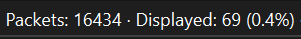
\includegraphics[width=1\linewidth]{img/1.png}
	\caption{received udp packet count}\label{fig:1}
\end{figure}

\begin{figure}[htbp]
	\centering
	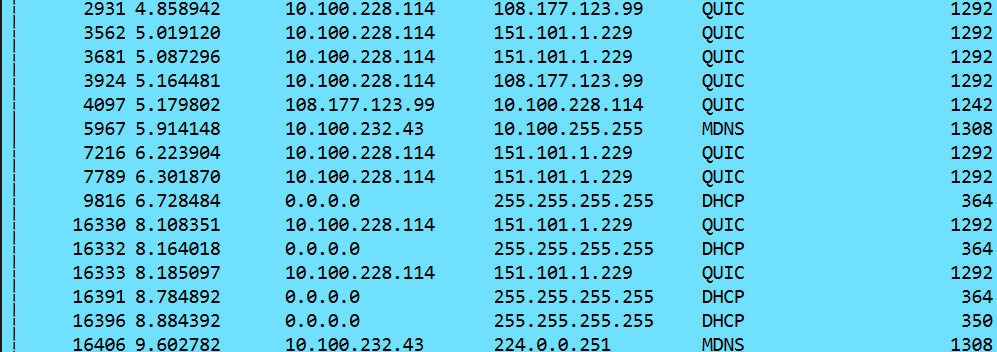
\includegraphics[width=1\linewidth]{img/2.png}
	\caption{UDP packet protocols}\label{fig:2}
\end{figure}

There were also many packets that were not necessarily related to the URL we
visited, such as a DNS query to \textit{watson.events.data.microsoft.com}. This
specific hostname is related to Windows telemetry.

\begin{figure}[htbp]
	\centering
	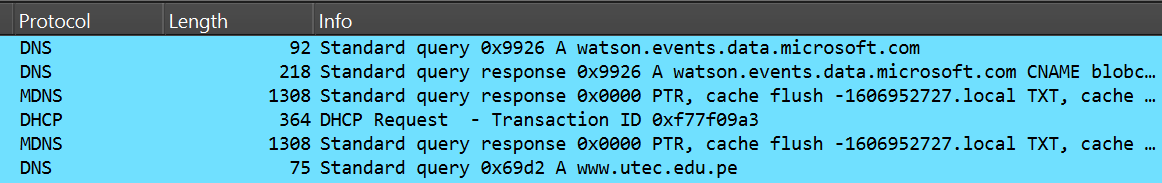
\includegraphics[width=1\linewidth]{img/3.png}
	\caption{Windows telemetry~\ensuremath{:(}}\label{fig:3}
\end{figure}

After that, we selected the first outgoing DNS packet going to
\textit{www.utec.edu.pe} to analyze its contents, which are displayed below.

\begin{figure}[htbp]
	\centering
	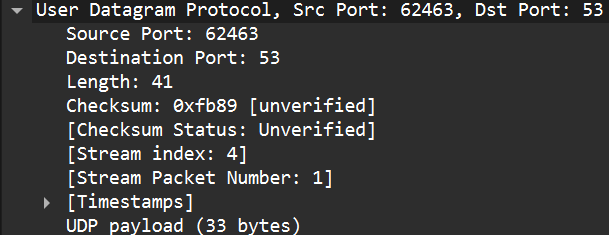
\includegraphics[width=1\linewidth]{img/4.png}
	\caption{www.utec.edu.pe packet info}\label{fig:4}
\end{figure}

The packet's main fields are:

\begin{itemize}
	\item Source/Destination Port: Port used for outgoing packet, destination port is the
	      default DNS port (53).
	\item Length: Total length of the UDP packet (41 bytes).
	\item Checksum: Value used to verify the integrity of the packet.
	\item Checksum Status: Indicates whether the checksum is correct or not.
\end{itemize}

The checksum status shown in the packet is ``Unverified'', which means that the
packet's correctness was not checked. This either means that Windows 11 is not
checking the integrity of outgoing and incoming packets, or that Wireshark is
not able to verify it (most likely).

After looking around in Wireshark settings, we found a way to enable checksum
validation for UDP packets. Enabling it updated the packet info field:

\begin{figure}[htbp]
	\centering
	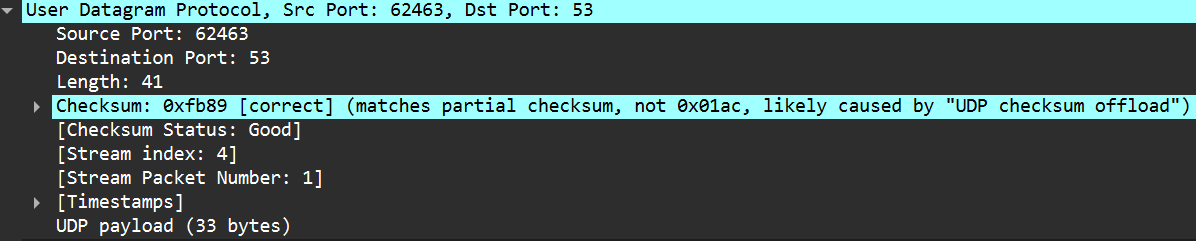
\includegraphics[width=1\linewidth]{img/5.png}
	\caption{Wireshark checksum validation}\label{fig:5}
\end{figure}

The checksum status is now ``Correct'', although it displays a message saying
that it matches the partial checksum, and that it's probably due to ``UDP
checksum offload''. A little research on this shows that it's a feature
integrated into modern NICs (Network Interface Cards) that allows them verify
the checksum, instead of having the CPU do it. This improves performance, but
it can cause small mismatches, like we saw in Wireshark.

Comparing the UDP packet info with a TCP packet, we can immediately see some
differences. There are stream indexes, TCP segments information, and most
importantly, \textbf{acknoledgment} related fields. This shows one of TCP's
particular features, handshakes.

Handshakes are a way for TCP to ensure that both servers are able to
communicate without issues. Server A sends a handshake packet to server B,
which server B then responds to with another handshake and an acknoledgment.
Finally, when server A receives it, it sends a final handshake and information
transfer can begin.

\begin{figure}[htbp]
	\centering
	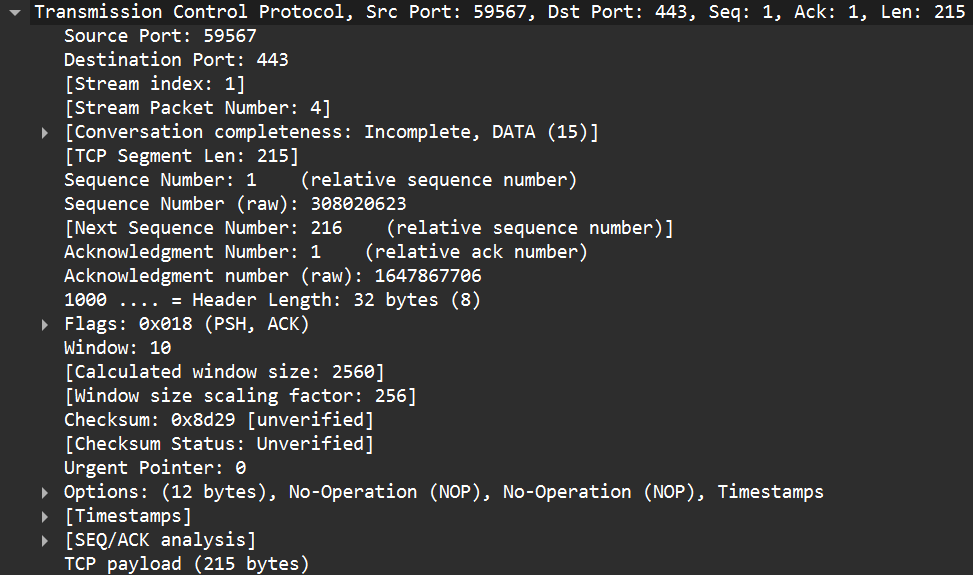
\includegraphics[width=1\linewidth]{img/6.png}
	\caption{TCP info}\label{fig:6}
\end{figure}

\subsubsection{Using nslookup}

Now again we set Wireshark's filter to display UDP only, but now visiting
\textit{www.cisco.com}, the total UDP packet count was approximately 4. All of them have de DNS protocol.\@

\begin{figure}[htbp]
	\centering
	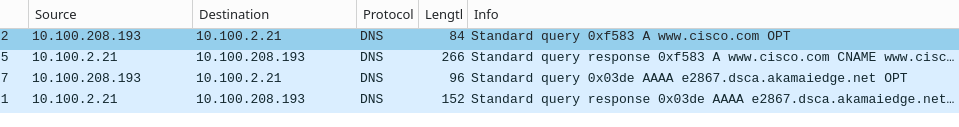
\includegraphics[width=1\linewidth]{img/7.png}
	\caption{received udp packet count}\label{fig:7}
\end{figure}

\begin{figure}[htbp]
	\centering
	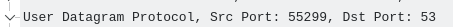
\includegraphics[width=1\linewidth]{img/8.png}
	\caption{first query package ports}\label{fig:8}
\end{figure}

\begin{figure}[htbp]
	\centering
	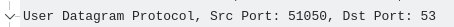
\includegraphics[width=1\linewidth]{img/9.png}
	\caption{second query package ports}\label{fig:9}
\end{figure}

The reason why nslookup generates UDP traffic is because it searches for dns servers, dns is the network service who relies on this context. The source and destnation ports of the packages are 55299, 51050 and 53. This shows that DNS default port is 53. The length of the DNS request is about 50 bytes, while the length of the response is higher than 100 bytes, being of course biggger than the request because it contains something, it's transporting.

\begin{figure}[htbp]
	\centering
	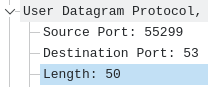
\includegraphics[width=1\linewidth]{img/10.png}
	\caption{first query package ports}\label{fig:10}
\end{figure}

\begin{figure}[htbp]
	\centering
	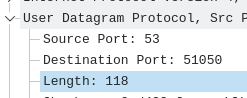
\includegraphics[width=1\linewidth]{img/11.png}
	\caption{second query package ports}\label{fig:11}
\end{figure}

\begin{figure}[htbp]
	\centering
	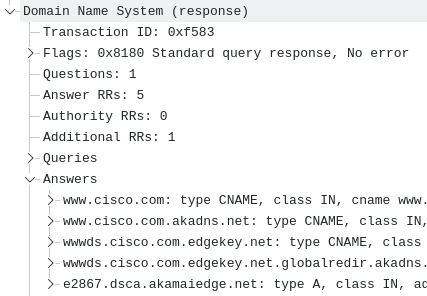
\includegraphics[width=1\linewidth]{img/12.png}
	\caption{second query package ports}\label{fig:12}
\end{figure}


The query was resolved successfully because the responses have the answers xd. Probably DNS uses UDP because its faster and thats needed in the context of web traffic, like web pages for example.


\cite{rfc1034}


\subsection{Second Experience}

\subsubsection{IPv6}
wasa

\subsubsection{Practical Exercise}

Theoretical questions:

\begin{itemize}
    \item 10.15.32.200/8: class A, NA 10.0.0.0, BA 10.255.255.255
    \item 172.20.45.7/12: class B, NA 172.16.0.0, BA 172.16.255.255
    \item 192.168.10.25/16: class C, NA 192.168.0.0, BA 192.168.255.255
\end{itemize}

After choosing the first TCP packet, we expanded and examined the IPv4 section.

\begin{figure}[htbp]
    \centering
    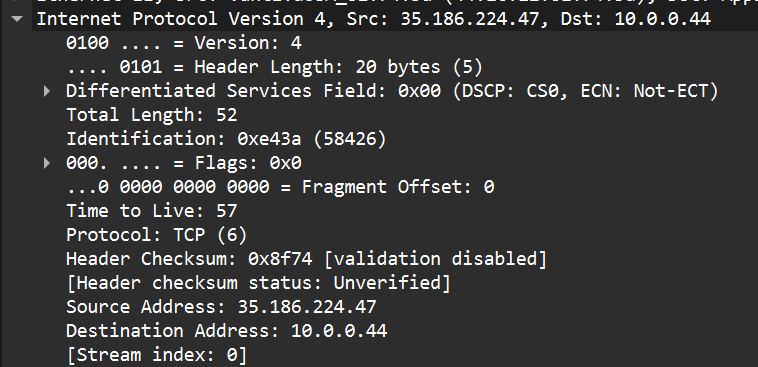
\includegraphics[width=1\linewidth]{img/2/6_1.png}
    \caption{TCP packet's IPv4 section}\label{fig:exp2_6_1}
\end{figure}

The first octet shows that both the source address \texttt{35.186.224.47} and
the destination address \texttt{10.0.04} belong to the A class.

Given that both addresses belong to the same class, and the last 3 octets are
different, we can infer a subnet mask of \texttt{255.0.0.0}.

The destination address might be a private one, as it follows the
\texttt{10.0.0.0/8} default pattern.

Finally, the TTL value of 57 might indicate that the device sending the packet
has a Linux OS.

\newpage{}
\subsection{Third Experience}

In this experience, we captured and analyzed the TCP packets sent to a
\texttt{gaia.cs} server after uploading a text file containing an ASCII copy of
Alice in Wonderland.

\subsubsection{Bulk TCP Transfer}

The three-way handshake is a way of establishing a connection between two PCs.
It makes sure that:

\begin{itemize}
	\item Sender is able to communicate with the receiver
	\item The receiver is able to listen
	\item The sender is able to listen to the receiver's response
\end{itemize}

After sending the text file to the server, we analyzed the first three
handshake packets.

\begin{figure}[htbp]
	\centering
	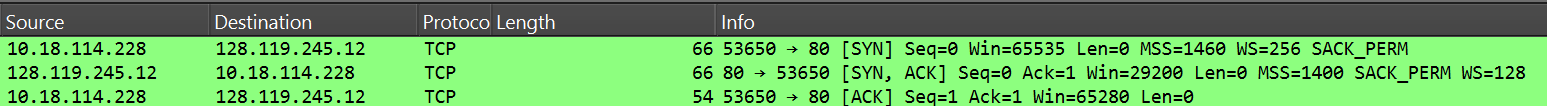
\includegraphics[width=1\linewidth]{img/third_experience/1.png}
	\caption{}\label{fig:3_1}
\end{figure}

By observing the contained headers, we can see that:

\begin{itemize}
	\item The first packet is a SYN (synchronize) packet sent from the sender to the
	      receiver. Its sequence value is 0.
	\item Shortly after, the receiver responds with a SYN-ACK (synchronize-acknowledge)
	      packet. The ACK value was set to 1, which means that the receiver acknowledged
	      the sender's sync request.
	\item Finally, the sender responds with an ACK package and sequence value set to 1.
	      This means that the connection was established, and the sequence step (stage)
	      is now 1 (data transfer enabled).
\end{itemize}

Thanks to this short analysis, we can see that the ACK value is set to 1 after
the receiver \textbf{ACKnowledges} the sender's request. It's a way of
confirming the connection request.

The ports used for communication were:

\begin{itemize}
	\item Sender SYN:\@ 53650 to 80
	\item Receiver ACK:\@ 80 to 53650
	\item Sender ACK:\@ 53650 to 80
\end{itemize}

Disabling capture of HTTP packets in Wireshark stops them from showing up in
the Wireshark dashboard.

Clicking on any TCP packet and following the stream shows the entire
communication sequence with the sent and received packets in a readable format.
On the bottom left, we can see that 18 packets were needed to send the entirety
of the text content.

The sequence number of a TCP packet is a number that identifies the order of
the packet being sent. It's sent according to the previous' packet sequence
number length.


\subsection{Report Research}

This subsection answers the report research questions, and provides additional
information that would otherwise clutter the main report.

\subsubsection{Risks of using UDP}
% What are the potential risks or vulnerabilities of using UDP in a network?
% Did you observe any unusual or potentially malicious UDP traffic?
Because UDP offers speed and low overhead, it can be used to send large numbers
of packets quickly, which can overwhelm servers without sufficient resources or
control for this types of situtations. This makes UDP an easy choice for DDoS
attacks, where attackers send large volumes of packets, and UDP's lack of
handshakes offer no limitation on the sender side~\cite{mirkovic2004taxonomy}.
During our experiences, we did not observe any particularly suspicious UDP
traffic, but the risk still remains.

\subsubsection{Detecting suspicious UDP traffic with Wireshark}
% How could an administrator use Wireshark to detect suspicious UDP
% behaviour, such as a port scan or DDoS attemp?
There are several types of port scanning techniques, and as such, different
ways to detect them. For this particular example, we'll analyze the classic SYN
scan, which sends SYN packets to several ports on the target computer. If the
port is open, the sender will receive a SYN-ACK, while close ports will usually
send a RST packet~\cite{rfc3360}. \\

Using Wireshark, an admin could filter SYN packets, and check if they were sent
to multiple ports in a short time frame. They could also check for high RST
packet frequency, which could indicate that several closed ports were
scanned.\\

In the case of a DDoS attempt, an admin could filter UDP packets by IP, and
check for a single repeating source IP.\@If the attack comes from multiple
sources, however, this task becomes more difficult.

\subsubsection{Testing TCP congestion mechanisms}
% abrir netflix, yt, etc
% plot wireshark capture and observe the window behaviour and tcp
% sequencing behaviour
% is there any packet loss?

\section{Conclusion}

\section*{Conclusion}

In this report, we utilized Wireshark to analyze the content and behaviour of
HTTP packets in a series of small experiments. By observing the HTTP GET
requests and responses, we understood how communication between hosts and
servers happens, as well as the different HTTP versions, status codes, and
headers.

The lab experience with long documents and embedded objects showed how data
transmitted via TCP is segmented into packets and how browsers handle multiple
resource requests.

On the other hand, the authentication section helped us see how credentials are
transmitted in a slightly ``secure'' way by using base64 encoding.

To summarize, these experiences reinforced newly learned computer networks
concepts, and also highlighted the importance Wireshark as a packet analysis
tool.

% if have a single appendix:
%\appendix[Proof of the Zonklar Equations]
% or
%\appendix  % for no appendix heading
% do not use \section anymore after \appendix, only \section*
% is possibly needed

% use appendices with more than one appendix
% then use \section to start each appendix
% you must declare a \section before using any
% \subsection or using \label (\appendices by itself
% starts a section numbered zero.)
%

% \appendices
% \section{Proof of the First Zonklar Equation}
% Appendix one text goes here.

% you can choose not to have a title for an appendix
% if you want by leaving the argument blank
% \section{}
% Appendix two text goes here.

% use section* for acknowledgment
% \section*{Acknowledgment}

% The authors would like to thank\ldots

% Can use something like this to put references on a page
% by themselves when using endfloat and the captionsoff option.
\ifCLASSOPTIONcaptionsoff{}
\newpage
\fi

% trigger a \newpage just before the given reference
% number - used to balance the columns on the last page
% adjust value as needed - may need to be readjusted if
% the document is modified later
%\IEEEtriggeratref{8}
% The "triggered" command can be changed if desired:
%\IEEEtriggercmd{\enlargethispage{-5in}}

% references section

% can use a bibliography generated by BibTeX as a .bbl file
% BibTeX documentation can be easily obtained at:
% http://mirror.ctan.org/biblio/bibtex/contrib/doc/
% The IEEEtran BibTeX style support page is at:
% http://www.michaelshell.org/tex/ieeetran/bibtex/
%\bibliographystyle{IEEEtran}
% argument is your BibTeX string definitions and bibliography database(s)
%\bibliography{IEEEabrv,../bib/paper}
%
% <OR> manually copy in the resultant .bbl file
% set second argument of \begin to the number of references
% (used to reserve space for the reference number labels box)
\bibliographystyle{IEEEtran}
\bibliography{references}

% biography section
% 
% If you have an EPS/PDF photo (graphicx package needed) extra braces are
% needed around the contents of the optional argument to biography to prevent
% the LaTeX parser from getting confused when it sees the complicated
% \includegraphics command within an optional argument. (You could create
% your own custom macro containing the \includegraphics command to make things
% simpler here.)
%\begin{IEEEbiography}[{\includegraphics[width=1in,height=1.25in,clip,keepaspectratio]{mshell}}]{Michael Shell}
% or if you just want to reserve a space for a photo:

% \begin{IEEEbiography}{Michael Shell}
%   Biography text here.
% \end{IEEEbiography}

% if you will not have a photo at all:
% \begin{IEEEbiographynophoto}{John Doe}
%   Biography text here.
% \end{IEEEbiographynophoto}

% insert where needed to balance the two columns on the last page with
% biographies
%\newpage

% \begin{IEEEbiographynophoto}{Jane Doe}
%   Biography text here.
% \end{IEEEbiographynophoto}

% You can push biographies down or up by placing
% a \vfill before or after them. The appropriate
% use of \vfill depends on what kind of text is
% on the last page and whether or not the columns
% are being equalized.

%\vfill

% Can be used to pull up biographies so that the bottom of the last one
% is flush with the other column.
%\enlargethispage{-5in}

% that's all folks
\end{document}

